% Activate the following line by filling in the right side. If for example the name of the root file is Main.tex, write
% "...root = Main.tex" if the chapter file is in the same directory, and "...root = ../Main.tex" if the chapter is in a subdirectory.
 
%!TEX root =  ../Thesis.tex

\chapter[ATLAS Detector]{CERN, the LHC Accelerator and the ATLAS Detector}




\section{Introduction}

%http://home.web.cern.ch/about/accelerators
\section{CERN and the Large Hadron Collider}
\label{sec:cern_lhc}
The European Center for Nuclear Research (CERN) is a scientific complex in Geneva, Switzerland that was established in the years following World War II.  Its focus is experimental particle physics, in particular the Large Hadron Collider (LHC), although it also houses a theoretical physics department and numerous other experiments relating to the fundamental particles and their interactions.  

The LHC is the accelerator that serves as the centerpiece of CERN's scientific program.  The accelerator is an RF-driven circular sychrotron located in an underground tunnel with a circumference of 27 km, and when it is running, accelerates and collides two proton beams (sometimes two lead ion beams) at four points around the accelerator ring.  At each of these collision points is a detector designed to measure the particles resulting from the collisions: CMS, LHCb, ALICE, and the experiment where the data for this thesis was collected, ATLAS.

The LHC is the last and most powerful in a series of staged accelerator complexes, which in combination accelerate protons from rest to an energy of 4 TeV as of 2012.  Since there are 2 beams that collide head-on, the total center-of-mass energy is 8 TeV.  The first step in the process is the proton source, where hydrogen atoms are subjected to an electric field that separates the protons from the electrons.  Then the protons are accelerated by a 90kV field and focused, then sent to the linear collider.  From this point forward, all the accelerators use radio frequency (RF) electromagnetic waves to impart energy to the protons.  

The linear accelerator brings the protons up to an energy of 50 MeV, then they go to the Proton Synchrotron Booster (up to 1.4 GeV), and then the Proton Sychrotron (25 GeV).  Then the protons are passed to the Super Proton Synchrotron, where they reach an energy of 450 GeV, and finally the beam is split into half and each half is injected into the LHC going a different direction.  Figure ~\ref{fig:accelerator_complex} shows all the major accelerators at the CERN site.

%%% CERN accelerator figure
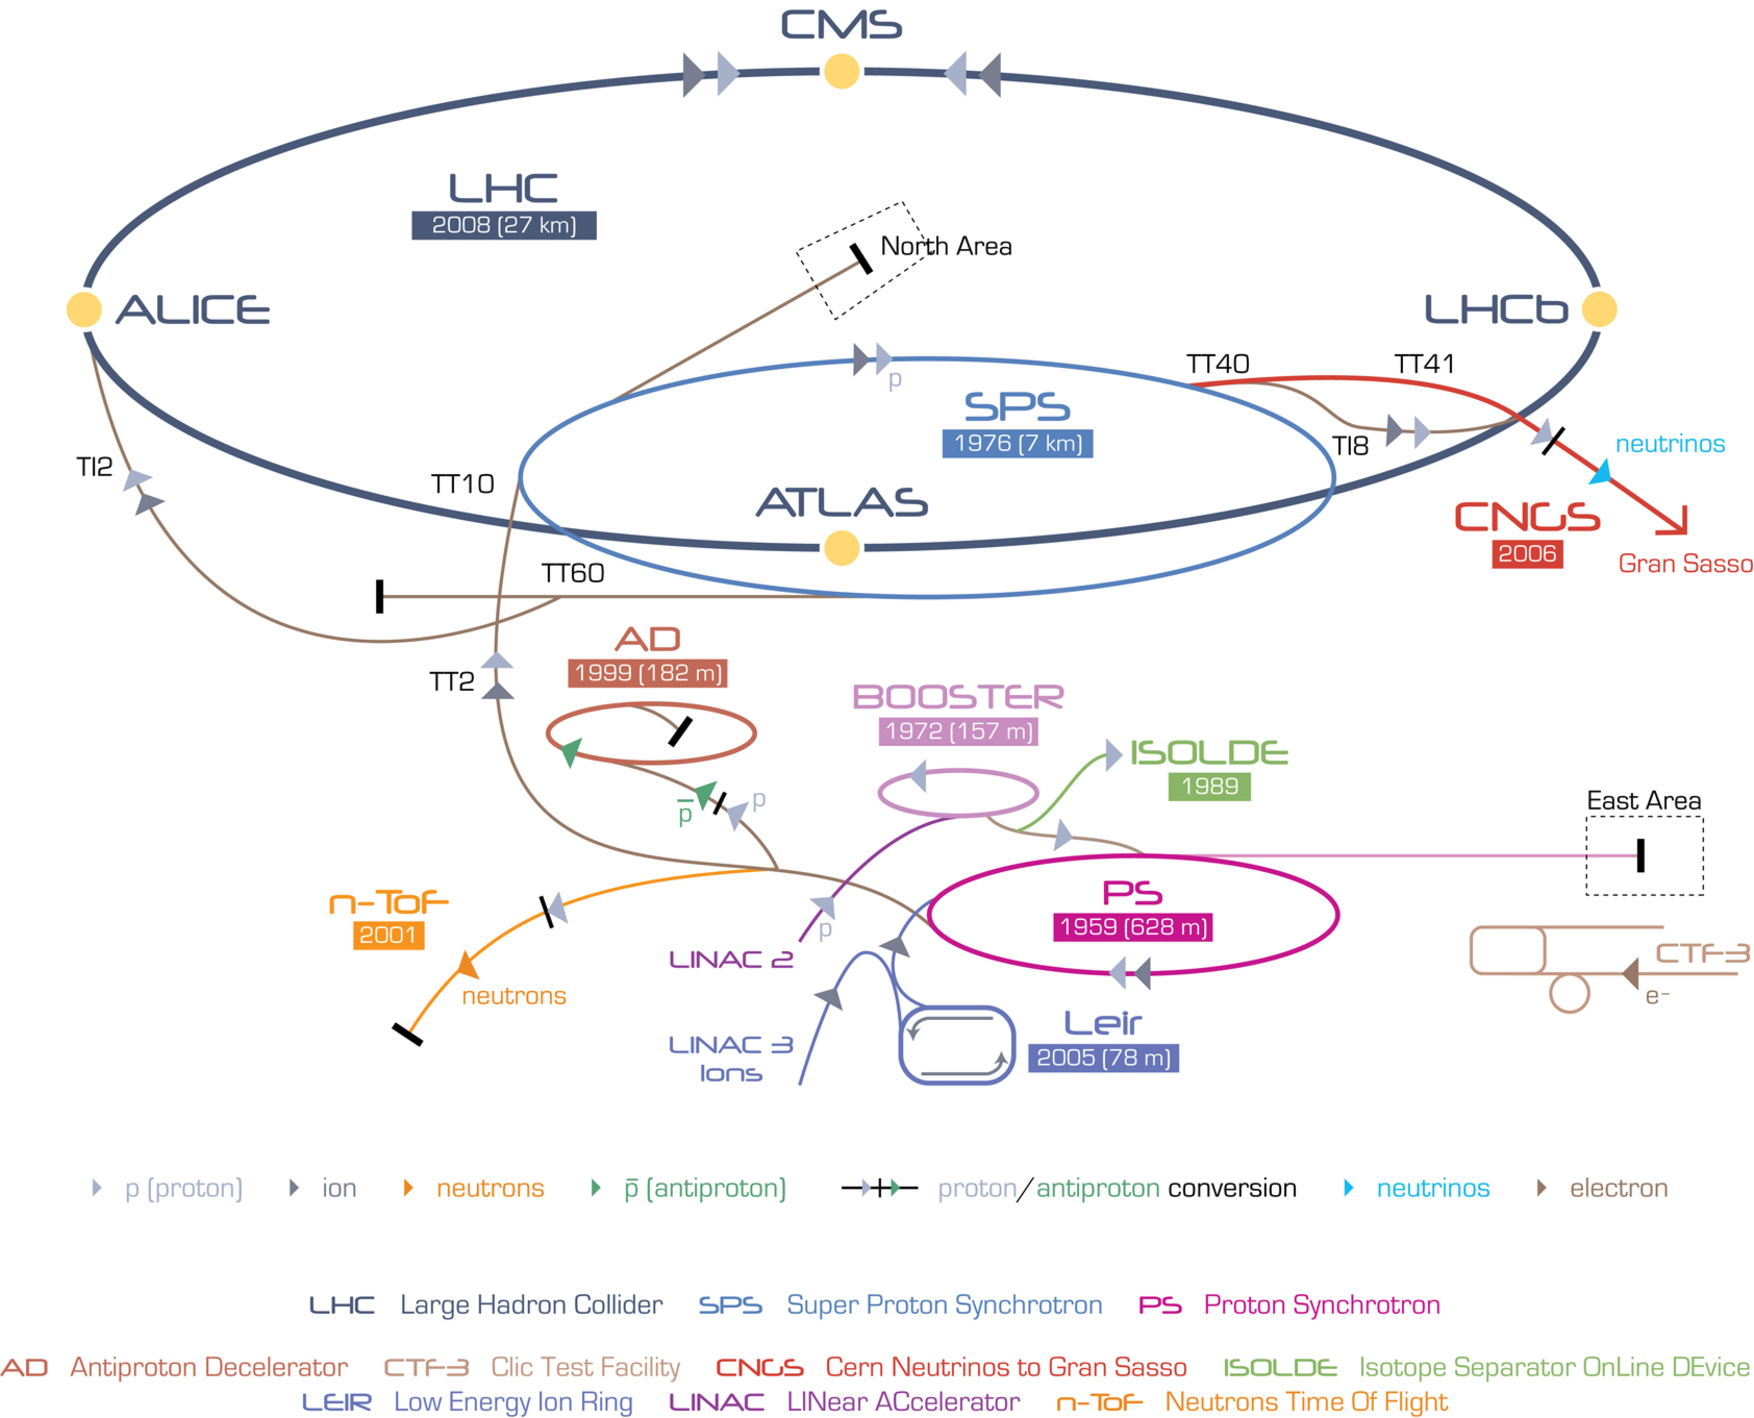
\includegraphics[width=0.5\textwidth]{/Users/caitlinmalone/Documents/Thesis/ATLASDetector/images/Cern-Accelerator-Complex.pdf}\label{fig:accelerator_complex}
%%% lumi in 2010, 2011 and 2012
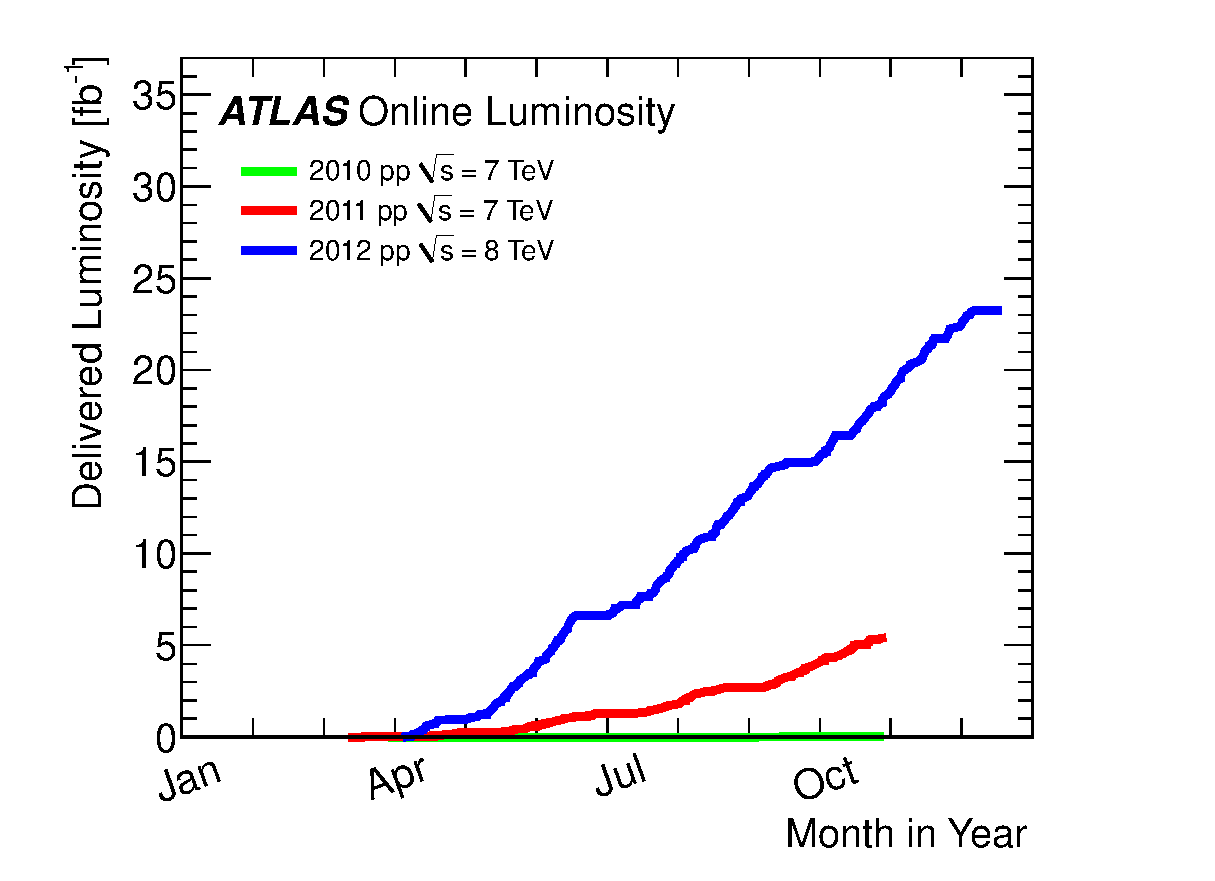
\includegraphics[width=0.5\textwidth]{/Users/caitlinmalone/Documents/Thesis/ATLASDetector/images/intlumivsyear.eps}\label{fig:lumi_vs_year}


Once the beams are in the LHC, they are accelerated over the course of about 20 minutes up to the full collision energy of 4 TeV per beam.  Then the beams are focused at each of the 4 interaction points, and carefully steered into position so that head-on collisions commence.  The protons are arranged in bunches within the beams, with each bunch 50 ns away from its neighbors, so that the collision frequency within the detectors is 20 MHz.  

The LHC first turned on in 2008, but within days had to shut down following a catastrophic failure of the bus bar between superconducting magnets.  It restarted in 2009 at 7 TeV, half the design energy of 14 TeV, and the first run for physics was performed in 2010, with a total dataset size of 36 inverse picobarns.  The progress in 2011 was dramatic, as the beam intensity was steadily increased over the course of the run to create an exponential increase of the luminosity recorded, and at the end of 2011 the total dataset size was about 5 inverse femtobarns.  The progress continued in 2012, with a slightly increased energy of 8 TeV, culminating in the 4 July 2012 announcement of the discovery of a new particle, later confirmed to be the long-sought Higgs boson.  At the end of 2012, the LHC commenced a 2-year shutdown to complete upgrades and repairs, with the intention of starting up again in 2015 at 13 TeV and 25 ns spacing between bunch crossings.

As Figure \ref{fig:lumi_vs_year} shows, the luminosity delivered in 2010, 2011 and 2012 increased dramatically from year to year.  This increase in data enabled more sensitive analyses and the Higgs discovery, but did not come for free.  In particular, over the course of this period, the number of protons and the bunch emittance were tuned to increase the number of collisions per bunch crossing, and thus the instantaneous luminosity.  An important consequence was that the pileup increased dramatically, creating a very busy environment where identification and reconstruction of physics objects becomes more challenging.  The implications of pileup both in general and in this analysis will be detailed in further chapters.


It is then the job of the ATLAS detector, and its readout system, to measure and record the particles that result from these collisions.  The detector is constructed of several main subsystems, each of which is designed to make certain types of measurements of certain types of particles.  The main layers of the detector are the inner detector, the hadronic and electromagnetic calorimeter, and the muon system.


\section{The ATLAS Coordinate System}
The ATLAS detector is situation at Point 1 of the LHC ring.  Since the detector has a cylindrical shape, polar coordinates are the most natural basis for describing its geometry.  The radial direction (usually notated ``r'') is defined as the vector originating at the interaction point, in the middle of the detector, and pointing transverse to the beamline.  The azimuthal angle $\phi$ and the polar angle $\theta$ complete the coordinate system, although in practice it is more common to use pseudorapidity $\eta$ instead of $\theta$.  Pseudorapidity has the advantage of being a quantity that is Lorentz-invariant under boosts longitudinal to the incoming beams (in a hadron collider, the longitudinal component of the momentum of the incoming partons is not known).  The definition of pseudorapidity $\eta$ is

\begin{equation}
\eta = -ln(tan( \frac{\theta}{2} ))
\end{equation}

Since the proton is a composite particle, made of three quarks and an indeterminate number of gluons, even if the proton has a known energy, its constituent partons can have a wide range of energies.  In general, then, the exact collision energy can vary from event to event, and outgoing particles can be boosted forward in $\eta$.  However, energy is conserved in the $\phi$ dimension, so transverse energy and momentum ($E_T$ and $p_T$, respectively) should add up to zero in events where there are no particles escaping detection.

\section{Particle Detection and Identification}


\section{Inner Detector}
The innermost layer of the ATLAS detector is the tracker, which provides precision measurements of the trajectories of charged particles.  As a charged particle traverses the layers of the tracker, it ionizes the detector material which creates small electrical signals that can be amplified and read out by the system.  These so-called ``hits'' are combined during reconstruction into tracks, which represent the paths of particles like electrons, muons, and charged pions in the detector.

The information from the tracker is used in particular to determine the transverse momentum (p$_T$) of charged particles, and to perform particle identification.  The tracker consists of three primary subsystems: the pixels, semiconductor tracker (SCT), and transition radiation tracker (TRT).  A charged particle created at or near the interaction point would typically travel through all three subsystems, creating some number of hits in each one.  On average, a track has 3 pixel hits, 8 hits in the SCT (4 double-sided hits) and about 34 hits in the TRT, with all the inner detector subsystems enclosed by a 2 tesla solenoidal magnetic field. 


\begin{figure}
	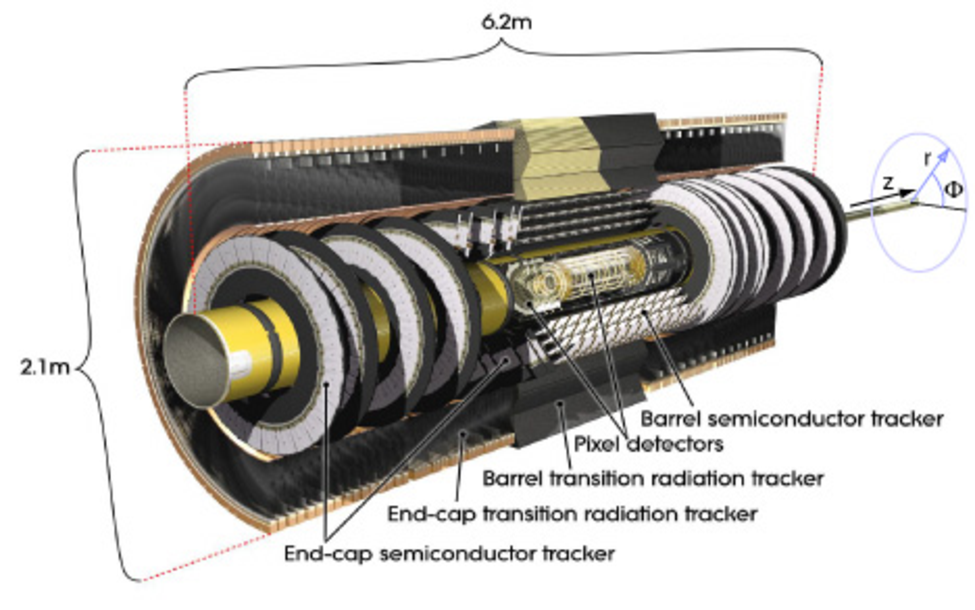
\includegraphics[width=0.8\textwidth]{/Users/caitlinmalone/Documents/Thesis/ATLASDetector/images/innerDetector.pdf}
	\label{fig:inner_detector}  
	\caption{A cutaway picture showing the main components of the ATLAS inner detector.}
\end{figure}


%http://cds.cern.ch/record/1290332/files/VERTEX%202010_015.pdf
\subsection{Pixel System}
\label{sec:pixel}
The pixel system sits physically closest to the beam line and interaction point.  It is built of silicon pixels that measure 50 x 400 micrometers each, which are organized into sensors.  Each sensor contains 46,080 pixels, and the sensors are arranged onto modules.  Each module contains 16 sensors, and there are 1744 modules total in the pixel system, organized into 3 layers each in the barrel and the two endcaps.  The pixel system in aggregate contains 80 million channels and measures about 1.4 meters long by 0.4 meters in diameter.

\begin{figure}
	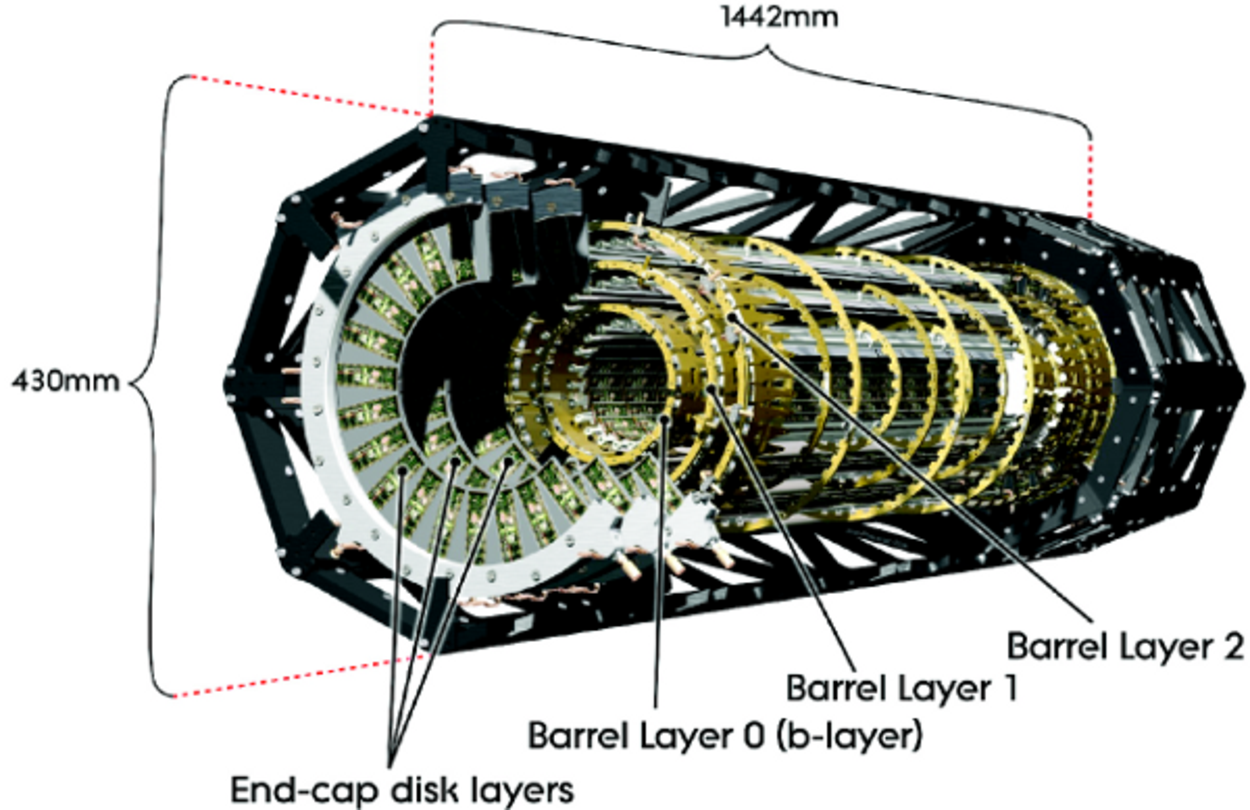
\includegraphics[width=0.8\textwidth]{/Users/caitlinmalone/Documents/Thesis/ATLASDetector/images/pixel_detector.pdf}
	\label{fig:inner_detector}  
	\caption{A picture showing the main layers of the ATLAS pixel detector.}
\end{figure}

% http://iopscience.iop.org/1748-0221/3/07/P07007/pdf/1748-0221_3_07_P07007.pdf
The pixel technology is designed to give high-precision measurements of the location and momentum of charged tracks.  A pixel module has two main components, the silicon sensor and the front-end chip, which are bump-bonded together.  When a charged particle traverses the sensor it ionizes silicon atoms, creating so-called electron-hole pairs, and then a bias voltage applied across the sensor causes the electrons and holes to drift to opposite sides of the sensor, where they can be read out by the front-end chips.  

The pixel readout is based on detecting and quantifying this ionization current.  A particle with greater momentum will create more electron-hole pairs and thus a longer readout pulse, which passes through a preamplifier and then a discriminator.  The discriminator is set with a tunable threshold number of electrons, typically a few thousand, and the signal metric is then the length of time for which the pulse was above that value (called ``time over threshold'', or TOT).  Having a threshold in place helps distinguish ionization current from leakage current, which occurs when the silicon does not have robust insulator characteristics and current begins to flow across the sensor even when there is no ionizing particle present.  One important effect of radiation damage to the pixel detector is that it damages the silicon, allowing for increases in leakage current up to 100 nA, so over the course of large radiation doses to the detector the thresholds sometimes have to be raised to compensate for the damaged material.  

Another important consideration when designing and constructing the pixel detector is the material budget of the system.  When a charged particle traverses the pixels, interacting with the silicon, its trajectory can change by virtue of these interactions as it undergoes multiple scattering or secondary interactions.  This can be a problem, for example, when reconstructing tracks--if a track has a kink from where it scattered off detector material, it will be more challenging to reconstruct the track or correctly measure its momentum.  These material effects are particularly important for the pixel detector, because they are the first layer of detector traversed by particles after they leave the collision point.  One way to mitigate these effects are to place high-material components, such as power supplies and readout electronics, in more forward regions so that they are not in the path of central tracks.  There are two figures of merit when evaluating the material budget of a system: the radiation length is the distance an electromagnetically interacting particle (such as an electron, positron or photon) travels before losing 1/$e$ of its energy to bremsstrahlung, which the interaction length is the mean distance traveled by a hadronically-interacting particle (such as a proton, neutron or pion) before undergoing an inelastic nuclear interaction.

%https://cds.cern.ch/record/1445527/files/ATL-COM-PHYS-2012-471.pdf
The pixel system all together provides fine resolution of the beamspot and surrounding area, which serves several important purposes.  First, since there are typically many hard p-p collisions in each bunch crossing, the pixels system has longitudinal resolution $z_0\sin\theta\approx$0.05-0.3 mm enables the reconstruction of multiple primary vertices that are typically separated by a few millimeters.  This is critical for controlling pileup in the high-luminosity LHC environment.  Second, the transverse resolution of 0.01-0.1 mm enables precision b-tagging for identification of bottom quarks.  B quarks typically have a lifetime of about 1ps, and since they are often created in high-p$_T$ collisions or come from the decay of heavy particles, they can have considerable $p_T$ and travel a few millimeters before decaying.  B-tagging algorithms typically look for evidence of secondary decay vertices that are displaced from the beamspot in the transverse direction.   


% useful thesis: http://www-pnp.physics.ox.ac.uk/~demirkoz/thesis.pdf
\subsection{Semiconductor Tracker (SCT)}
\label{sec:sct}
Like the pixels, the silicon microstrip tracker (SCT) is a silicon detector, although the geometry is distinctly different from the pixel geometry.  Since the SCT is at a farther radius from the interaction point than the pixels, it experiences a lower occupancy.  This allows for substantially larger detector elements, at a lower cost and using less material in the detector than if the same coverage were implemented in pixels, while maintaining 16 $\mu$m resolution of tracks in r$\Phi$ and 580 $\mu$m resolution in Z.   

The SCT geometry has some notable features.  The SCT consists of 8 layers of microstrips organized into 4 double-sided pairs, where the two members of each pair have an offset angle of 40 mrad.  The SCT has 4 barrel layers and 9 endcap disks, and the barrel modules are oriented with a tilt angle of about 11$^\circ$ angle relative to being perfectly tangential to $r\phi$.  Whereas the pixel reads out the TOT of a hit, the SCT has a binary readout: a hit is either recorded or not.



%https://indico.cern.ch/getFile.py/access?contribId=51&sessionId=8&resId=0&materialId=slides&confId=117804
\subsection{Transition Radiation Tracker}
\label{sec:trt}
The outermost inner detector layer is the transition radiation tracker, or TRT.  

The TRT uses gold-plated tungsten wires embedded in straw tubes of 4mm diameter filled with an Xe/O$_2$/Co$_2$ gas mixture, with a total of about 350,000 readout channels covering a pseudorapidity range out to $|\eta|<$2.0.  For a typical particle, the TRT will have about 30-35 hits with a hit precision of about 130$\mu m$.

One important objective of the TRT is to identify tracks from electrons by detecting transition radiation (hence the name transition radiation tracker).  Transition radiation occurs when an electron passes between regions with different dielectric constants; at the boundary between those regions, the electron can emit a photon which is then absorbed by the Xe gas and translates into a high-threshold hit in the detector.  Electrons can be distinguished from hadrons by the presence of many high threshold hits along the track.

 
% http://iopscience.iop.org/1742-6596/119/3/032014/pdf/1742-6596_119_3_032014.pdf
\subsection{Inner Detector Performance and Tracking}
\label{sec:id_perf}
Measurements from the pixel, SCT and TRT are combined in the track reconstruction.  There is a broad range of properties that tracks might have, so the inner detector has to be able to measure tracks with p$_T$ ranging from 150 MeV to 30 GeV or more.   

The main track reconstruction algorithm used at ATLAS is a version of the Kalman filter algorithm.  The track reconstruction begins with track seeds, which are collections of a few hits in the pixel subsystem that could plausibly be parts of tracks.  The advantage of starting with seeds, rather than attempting to find an entire track at once, is that seeds allow flexibility at the beginning of the search (when the track trajectory is the least known) while keeping computational costs down.  Once a seed has been identified, the Kalman fitter (as the ATLAS algorithm is called) projects where the next hit would be if there is truly a track present, and then looks for the presence of a hit at the predicted location in the next tracker layer.  If a hit is found there, the predicted trajectory of the particle may be refined and the next hit is predicted and sought, until all the detector layers have been traversed. If there is no hit present where one is predicted, the Kalman fitter can project two layers further, to allow for the possibility of a hole where the particle did not leave a hit for some reason. 

In high-pileup environments, the inner detector occupancy can be high which can make for two tracks that overlap, leaving a hit in the same place which must then be allocated to one or the other.  Dedicated ambiguity solving is implemented as a second stage in the track reconstruction, where the two candidate tracks are scored against each other via a reward/penalty scheme.  A good $\chi^2/DOF$ score is rewarded, a track with many holes on track or a low $\chi^2/DOF$ is penalized, with subdetector-specific weighting favoring the higher-precision silicon over the the lower-precision TRT. 


\section{Calorimeters}
The ATLAS detector has two calorimeter systems: the electromagnetic (EM) calorimeter, designed to measure the energy of electrons and photons, and the hadronic calorimeter, for measuring the energy of hadrons, jets, tau leptons and missing transverse energy.  

%http://www-library.desy.de/preparch/desy/proc/proc10-01/meng.pdf
%http://iopscience.iop.org/1742-6596/110/9/092007/pdf/jpconf8_110_092007.pdf
\subsection{Electromagnetic Calorimeter}
\label{sec:em_cal}
The electromagnetic (EM) calorimeter measures electrons and photons after they exit the tracking system.  The calorimeter consists of two major parts, the barrel and the endcaps; the barrel measures particles with $|\eta|<$1.475 and the endcaps measure particles with 1.375$<|\eta|<$3.2.  The calorimeter is a sampling calorimeter, with the passive showering material (lead) interleaved with active energy measurement material (liquid argon, or LAr).  An electron or photon will interact with the lead as it travels through it, creating an electromagnetic shower, which then propagates to the adjacent LAr layer, where it is measured and read out.

A notable feature of the EM calorimeter is the accordion geometry, which has several key characteristics.  First, the geometry enables complete coverage in $\phi$ without azimuthal cracks.  Second, the LAr sampling layer between lead layers is constant throughout the calorimeter barrel.  Third, a particle traveling through the calorimeter will generate approximately the same number of sampling instances (i.e. measurements) regardless of the direction in which it travels.  These pieces add up to a very uniform coverage of electromagnetic calorimetry.

The performance requirement for the resolution of the EM calorimeter is $\sigma_E/E=\frac{10\%}{\sqrt{E}}+$0.7\%, and a crucial part of reaching this resolution is precisely understanding the shape of the readout pulse.  The traversing particle produces an electromagnetic shower where the drift time of the particles in the shower cause a readout pulse that is roughly triangular in shape and typically 400 ns long.  This pulse is shaped by the readout electronics and the signal shape is simulated with Monte Carlo and calibrated using precisely known test pulses deposited into the readout chain.  However, as detailed below, the presence of multiple interactions per bunch crossing, known as pileup, has a significant effect in the calorimeters and is an important task for understanding jet energy.

%http://cds.cern.ch/record/1478440/files/ATL-TILECAL-PROC-2012-008.pdf
%http://arxiv.org/pdf/1305.0550v1.pdf
%http://cds.cern.ch/record/1393742/files/CERN-THESIS-2011-144.pdf
\subsection{Hadronic Calorimeter} 
\label{sec:h_cal}
The hadronic calorimeter measures the energy from hadrons, jets, taus and allows for a measurement of missing transverse energy.  The hadronic calorimeter, nicknamed the tile calorimeter because of its composition of scintillating tiles interleaved with steel plates.  The calorimeter is partitioned into four major subsections, two barrel sections and two extended barrel sections, allowing for measurements out to $|\eta|<$1.7.  In order to stop all particles from the collision, with the notable exception of muons, the hadronic calorimeter is about 7.4 radiation lengths ($\lambda$) thick.


\begin{figure}
	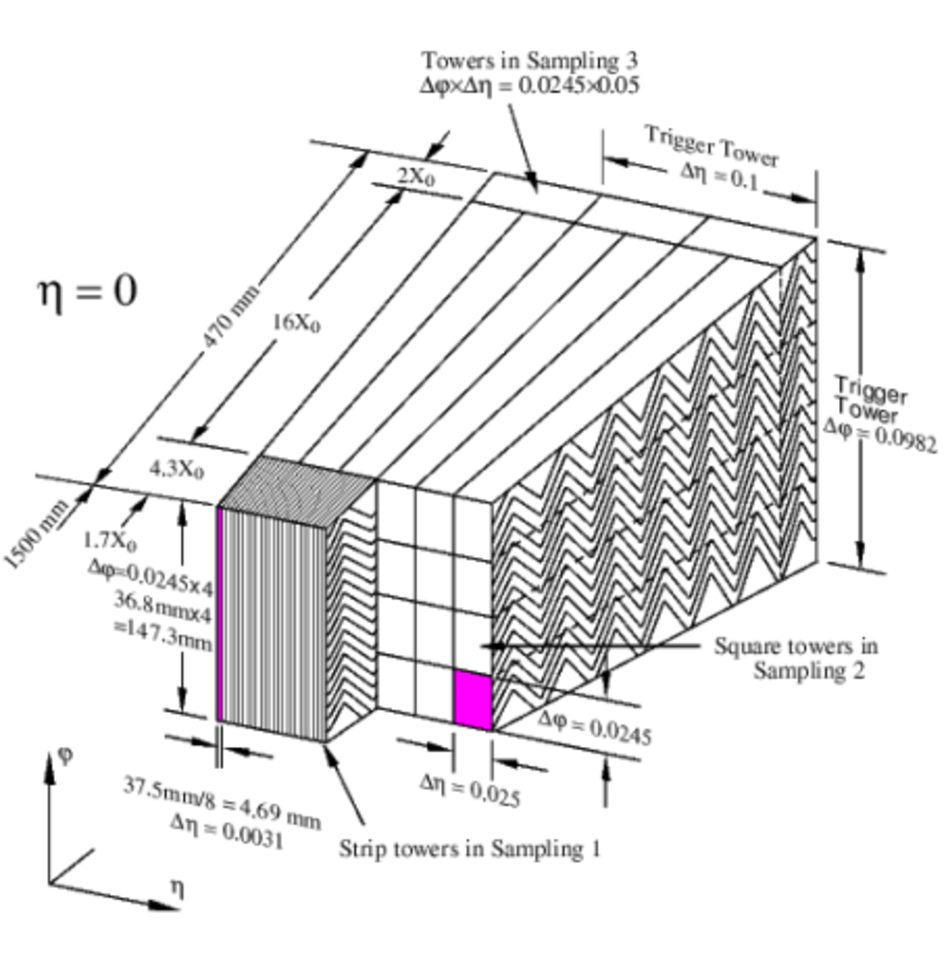
\includegraphics[width=0.8\textwidth]{/Users/caitlinmalone/Documents/Thesis/ATLASDetector/images/LArg_accordion.pdf}		\label{fig:lar}
	\caption{A depiction of a section of the LAr calorimeter.  The accordion structure of the towers is visible, as well as the three sampling layers}
	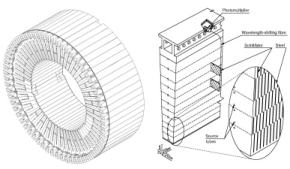
\includegraphics[width=0.8\textwidth]{/Users/caitlinmalone/Documents/Thesis/ATLASDetector/images/tile_cal.pdf}
	\label{fig:tile_cal}
	\caption{A depiction of the overall tile calorimeter, and a close-up view of one of its cells.}
\end{figure}


%http://iopscience.iop.org/1742-6596/331/2/022024/pdf/1742-6596_331_2_022024.pdf

\section{Muon System}
\label{sec:ms}
The ATLAS muon system is designed to measure the $p_T$ of muons with $p_T>$3 GeV, with 3\% resolution up to $p_T<$250 GeV and 10\% resolution up to 1TeV.  The system is composed of four different detector systems located within and around an air-core toroid magnet with a field of 1 Tesla.  Precision tracking in the barrel is done by Monitored Drift Tubes (MDT) and in the endcap by Cathode Strip Chambers (CSC).  Quick-readout triggering is done in the barrel by Resistive Plate Chambers (RPC) and in the endcap by Thin Gap Chambers (TGC).  

The muon system is often used in conjunction with the tracking of the inner detector, since a muon would be expected to create a track in both systems.  Also of particular interest for this thesis is when the muon system can be used in conjunction with the hadronic calorimeter, since b jets often decay semileptonically.  In this case, the muon from the b decay is often nearly colinear with the jet, so a muon that is ``matched'' with a deposit in the hadronic calorimeter can be used to identify and trigger on b decays.  

%%% ATLAS detector figure
\begin{figure}
	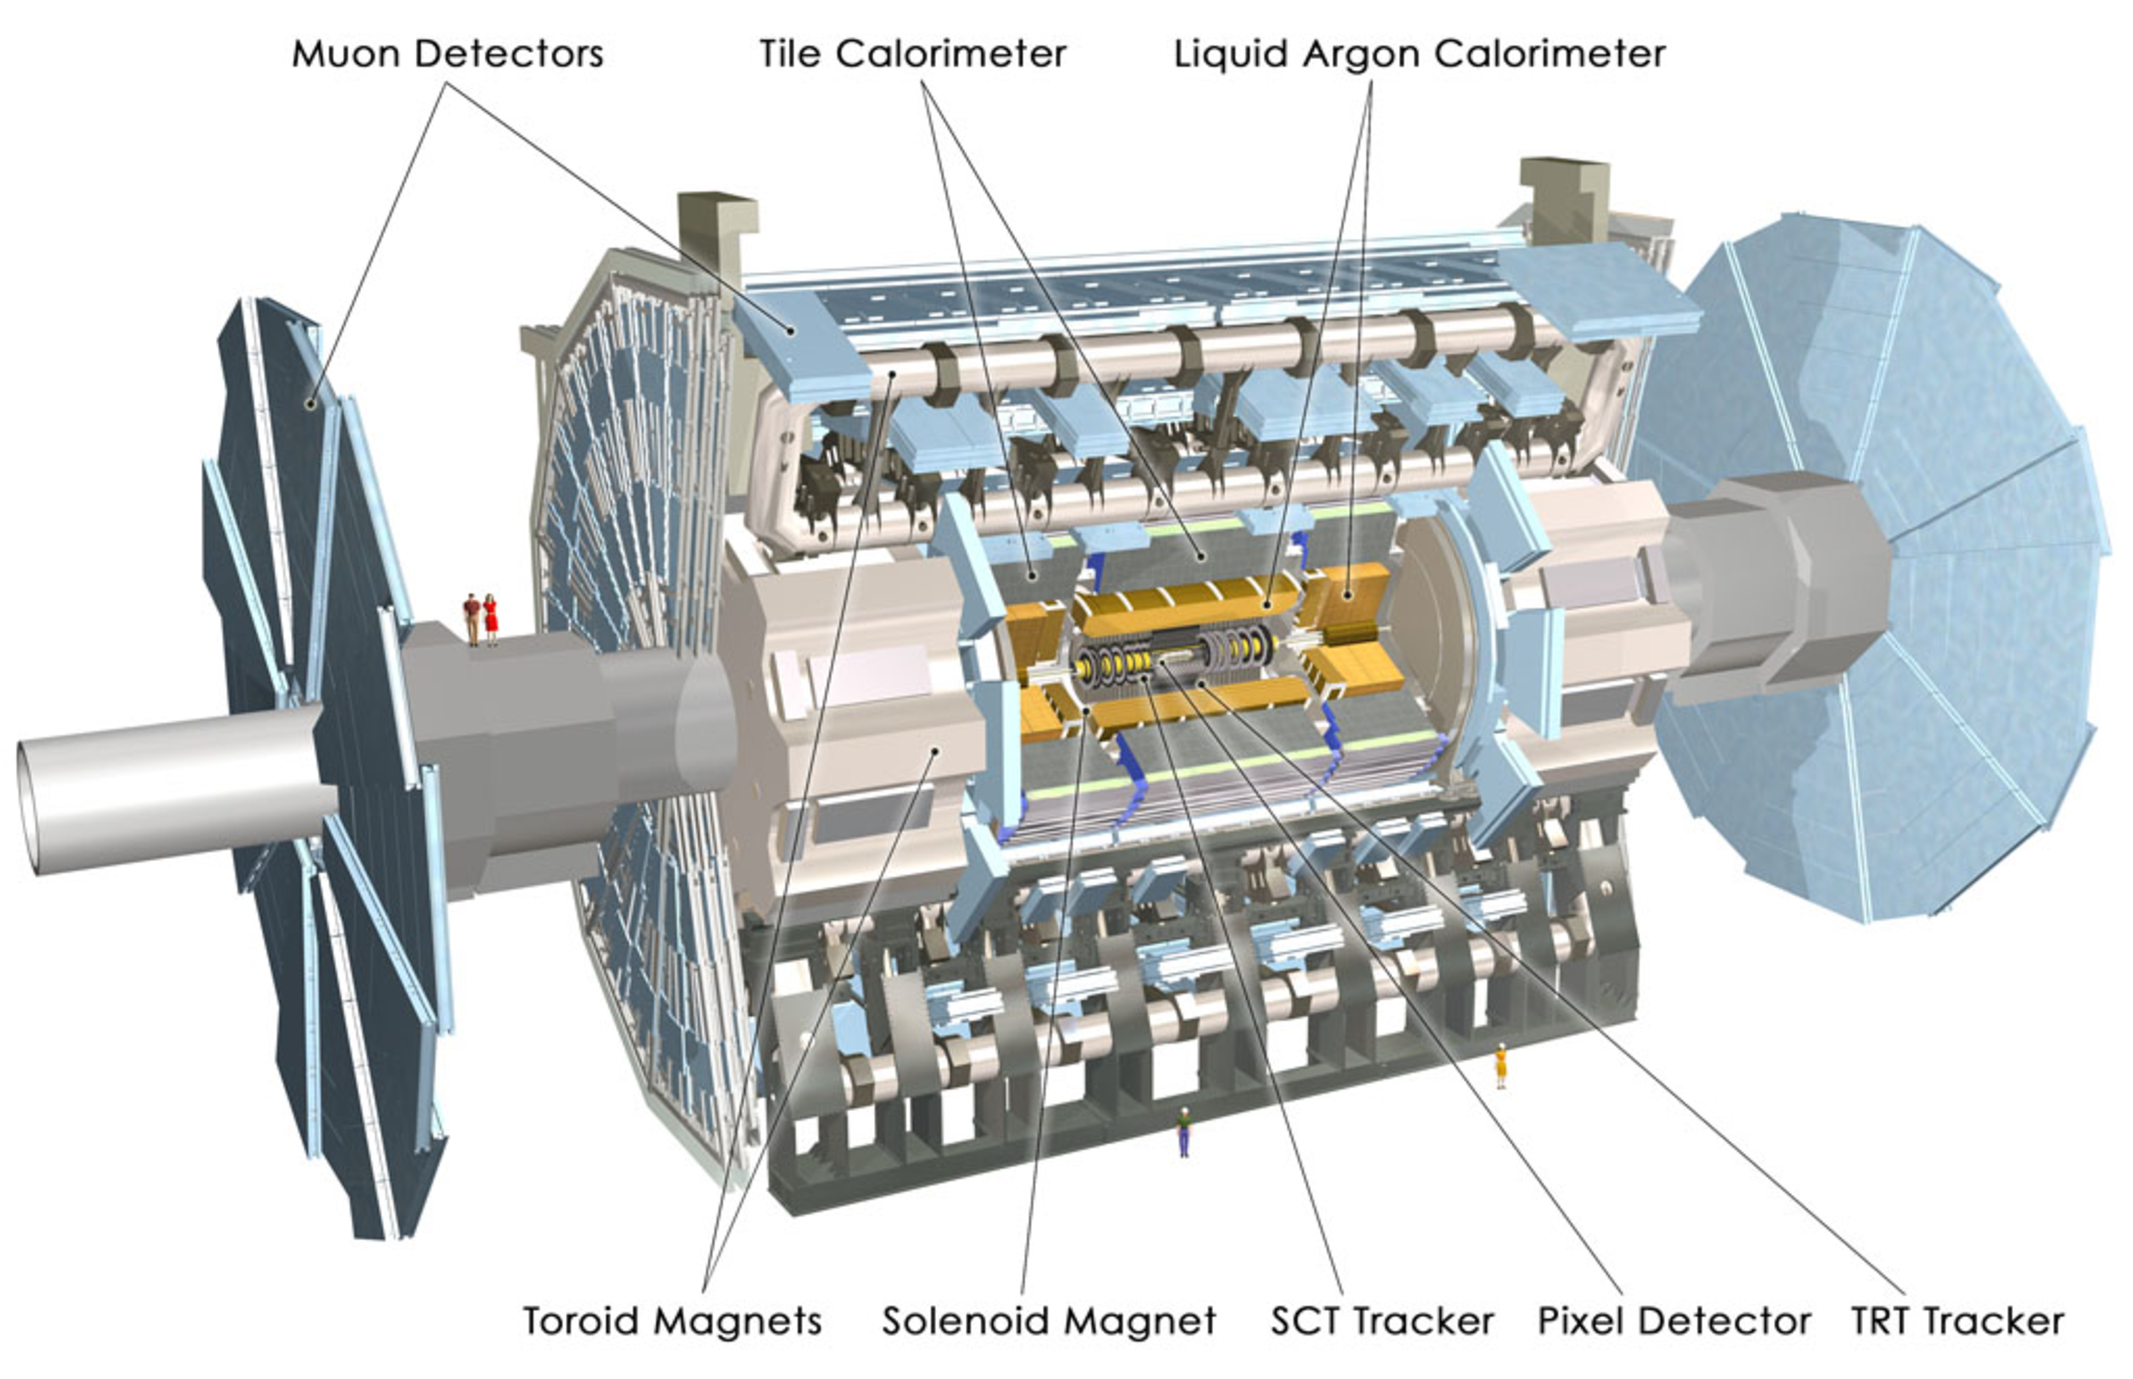
\includegraphics[width=\textwidth]{/Users/caitlinmalone/Documents/Thesis/ATLASDetector/images/AtlasDetectorLabeled.pdf}	\label{fig:detector}
\end{figure}

%http://www.slac.stanford.edu/econf/C0303241/proc/pres/502.PDF
%https://cds.cern.ch/record/1267390/files/ATL-DAQ-SLIDE-2010-087.pdf
\section{Trigger}
\label{sec:atlas_trig}
Although the LHC delivers 20 million bunch crossings per second to the ATLAS detector, the detector does not have the capacity in either storage space or readout bandwidth to record all these collisions.  The trigger has the task of selecting the most interesting 100 or so events per second, which are then fully reconstructed and recorded.  The trigger is a three-layer system, with a first level (L1) implemented solely in hardware, a second level (L2) that reconstructs ``regions of interest'' (RoI's) with special fast algorithms, and an event filter (EF) that reconstructs the full event with offline algorithms.  
 

The smallest piece of the trigger is a trigger object.  This is the signature left behind by a high-$E_T$ particle such as an electron, muon, b-quark, or photon (this is not an exhaustive list).  Many physics analyses look for signatures that have more than one physics object in them (for instance, multiple electrons, or a lepton plus jets), so multiple physics objects are often required in a single trigger.  If all of the objects are seen, the trigger is passed and the event moves forward in the data collection process.  This process repeats three times, once for each of the levels of the trigger--only those events which pass L1 move onto L2, and so on.   The chain of algorithms and decisions that are successively applied to a given trigger object are collectively called the trigger chain.  Then, groups of trigger chains that share common features are grouped together into trigger streams, where the primary trigger streams are JetTauEtMiss, EGamma, MinBias, and CosmicCalo.  The end result of this process is approximately 200 events per second (320 GB/s of data) being written to disk; the trigger rates and latency information can be found in Table \ref{tab:trigger_stats}.

  

% https://cds.cern.ch/record/1181075/files/05446486.pdf
\begin{table}
\begin{tabular}{c | c | c | c}
Trigger Level & Rate in Hz  & Latency  & Data Rate\\  \hline
None (Event rate) & 20 MHz  & no decision applied yet & 1600 TB/s \\
L1  & 75 kHz  &  $\sim$ 1$\mu s$  & 120 GB/s\\
L2  & 3 kHz    & $\sim$ 10 ms & 5 GB/s \\
EF  &  200 Hz  & $\sim$ 1 s & 320 MB/s \\
\end{tabular}
\end{table}
\label{tab:trigger_stats}


Of particular interest to this analysis are the jet thresholds and b-tagging applied in the trigger.  This will be outlined in greater detail in a later section, but we will introduce the ideas here.  As only 200 events per second get written to disk, the bandwidth has to be carefully allocated across triggers, and it is very expensive to keep a trigger that allows high rates of events to be written to data.  In an analysis such as this one, the physics objects coming from the signal (b-jets from a Higgs decay) are generally higher in p$_T$ than the background (continuum QCD processes) so one way to keep event rates reasonable in the face of rising luminosity is to place higher p$_T$ thresholds on the jets that fire the trigger.   

The thresholds increase with each trigger level, as the reconstruction algorithms become more accurate, so that a jet which is reconstructed with 145 GeV of p$_T$ at L1 might be required to have 170 GeV at EF in order to pass the full trigger.  Once the event is written to disk, it is subject to the full offline reconstruction and calibration so that the final p$_T$ of the jet might not be exactly the number measured at the trigger EF.  There is therefore a range of p$_T$ values, called the turn-on curve, where the trigger goes from rejecting all events to accepting all events.  Within the turn-on curve even a small change in the p$_T$ of a jet can have a dramatic difference in whether the jet fires a trigger accept, so this instability is mitigated by placing p$_T$ cuts on the trigger jets that require that their respective p$_T$ values are above the turn-on curve.  

The ATLAS trigger also allows for b-tagging of jets at L2 and EF.  For analyses that have b-jets in the final state, b-tagging in the trigger provides a tool for keeping rates low without pushing up jet p$_T$ thresholds.  B-tagging in the trigger introduces several challenges, though.  First, the online b-tagging algorithms have less time and information than the offline algorithms.  Second, a jet that passes an L2 b-tag will not necessarily pass an EF b-tag, and vice versa, so more work is required in understanding the correlations between tags at different trigger levels.  







